\section{Experimental results} \label{experimental_results}

% TODO: The third section shall report experimental results (e.g. training progress diagrams), describe interesting observations, and discuss the difficulties you faced and how you overcame them.

When starting the initial training process first a pre-training is executed which serves to fill the prioritized experience replay buffer with experiences from an expert rule-based agent and to pre-train the model itself to build up on some agent behavior already for the later training process. To not introduce a heavy bias the pre-training is stopped after 1.5k training games. \autoref{fig:pre-loss-1} shows the aggregated step loss per episode averaged after five episodes and \autoref{fig:pre-reward-1} the reward per episode averaged after five episodes. 

\begin{figure}[ht]
	\centering
	\begin{subfigure}[b]{0.49\textwidth}
		\centering
		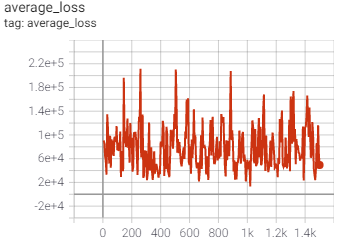
\includegraphics[width=\textwidth]{figures/training1-pre-loss.PNG}
		\caption{Pre-training loss}
		\label{fig:pre-loss-1}
	\end{subfigure}
	\hfill
	\begin{subfigure}[b]{0.49\textwidth}
		\centering
		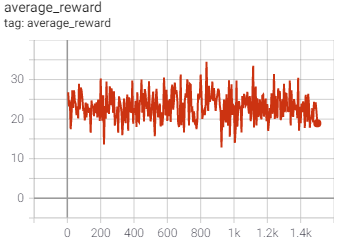
\includegraphics[width=\textwidth]{figures/training1-pre-reward.PNG}
		\caption{Pre-training average reward}
		\label{fig:pre-reward-1}
	\end{subfigure}
\end{figure}

When initiating the main training process with experiences gained from the dueling double DQN itself the following training curves can be experienced:

\begin{figure}[ht]
	\centering
	\begin{subfigure}[b]{0.49\textwidth}
		\centering
		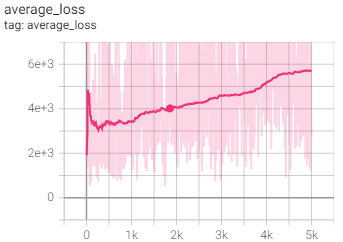
\includegraphics[width=\textwidth]{figures/training1-main-loss-smooth.PNG}
		\caption{Main-training loss}
		\label{fig:main-loss-smoothed-1}
	\end{subfigure}
	\hfill
	\begin{subfigure}[b]{0.49\textwidth}
		\centering
		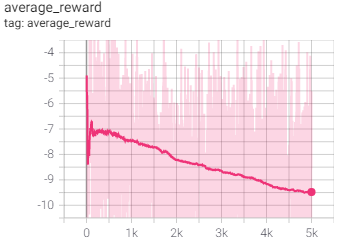
\includegraphics[width=\textwidth]{figures/training1-main-reward-smooth.PNG}
		\caption{Main-training average reward}
		\label{fig:main-reward-smoothed-1}
	\end{subfigure}
\end{figure}

The complete opposite of what was expected was observed, the loss increased whereas the average reward decreased. One possible explanation was a possible training bias introduced through the prioritized experience replay buffer towards transition with a high temporal difference error. Even if the gradient weighting factors were calculated and used to anneal the bias as proposed in the original paper, still this unintended behavior could be experienced. Therefore the training process was aborted after 5k episodes. 

The next generation of the model was trained on a normal experience replay buffer with the following results:

\begin{figure}[ht]
	\centering
	\begin{subfigure}[b]{0.49\textwidth}
		\centering
		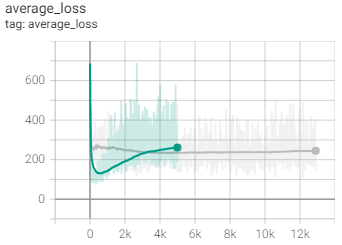
\includegraphics[width=\textwidth]{figures/training2-main-loss-smooth.PNG}
		\caption{Main-training loss}
		\label{fig:main-loss-smoothed-2}
	\end{subfigure}
	\hfill
	\begin{subfigure}[b]{0.49\textwidth}
		\centering
		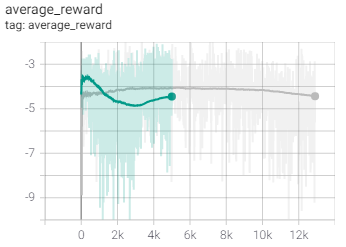
\includegraphics[width=\textwidth]{figures/training2-main-reward-smooth.PNG}
		\caption{Main-training average reward}
		\label{fig:main-reward-smoothed-2}
	\end{subfigure}
\end{figure}

Also, the initial exploration factor $\epsilon$ was increased to one to counter a possible pre-training bias and the maximum size of the experience replay buffer was decreased from 65.536 to 32.768 to train on more recent experiences. The green curve shows the training development until 5k episodes, which was then expanded to another 13k episodes plotted in the gray curve. 

Having done these changes results in a far lower training loss curve which converges to an average episode loss of 250 per five episodes. Also the reward curve seems to converge at an average loss of about minus four. Nevertheless, this average reward still is not what was expected and when looking at the actual agent behavior, the agent always chooses to wait. 
